%%%%%%%%%%%%%%%%%%%%%%%%%%%%%%%%%%%%%%%%%%%%%%%%%%%%%%%%%%%%%%%%%%%%%%%%%%%%%%%%
%2345678901234567890123456789012345678901234567890123456789012345678901234567890
%        1         2         3         4         5         6         7         8

\documentclass[letterpaper, 10 pt, conference]{ieeeconf}  % Comment this line out if you need a4paper

%\documentclass[a4paper, 10pt, conference]{ieeeconf}      % Use this line for a4 paper

\IEEEoverridecommandlockouts                              % This command is only needed if 
                                                          % you want to use the \thanks command

\overrideIEEEmargins                                      % Needed to meet printer requirements.

% See the \addtolength command later in the file to balance the column lengths
% on the last page of the document

% The following packages can be found on http:\\www.ctan.org
%\usepackage{graphicx}
\usepackage{graphics} % for pdf, bitmapped graphics files
\usepackage{epsfig} % for postscript graphics files
\usepackage{subcaption}
\usepackage[noadjust]{cite}
%\usepackage{mathptmx} % assumes new font selection scheme installed
%\usepackage{times} % assumes new font selection scheme installed
\usepackage{amsmath,amssymb,amsfonts} % assumes amsmath package installed
\usepackage{algorithm,algpseudocode}
%\usepackage{booktabs}
\usepackage{dsfont}
\usepackage{gensymb} % degree symbol

% format for theorems etc.
\newtheorem{thm}{\bfseries Theorem}
\newtheorem{lem}{\bfseries Lemma}
\newtheorem{cor}{\bfseries Corollary}
\newtheorem{prop}{\bfseries Proposition}
\newtheorem{rem}{\bfseries Remark}

% format for argmin, argmax
\newcommand{\argmax}{\operatornamewithlimits{argmax}}

% format for cross-reference
\usepackage[capitalize]{cleveref}
\crefname{equation}{eq.}{eq.}
\Crefname{equation}{Eq.}{Eq.}
\crefname{thm}{theorem}{theorems}
\Crefname{thm}{Theorem}{Theorems}
\crefname{lem}{lemma}{lemmas}
\Crefname{lem}{Lemma}{Lemmas}
\crefname{cor}{corollary}{corollaries}
\Crefname{cor}{Corollary}{Corollaries}
\crefname{prop}{proposition}{propositions}
\Crefname{prop}{Proposition}{Propositions}
\crefname{rem}{remark}{remarks}
\Crefname{rem}{Remark}{Remarks}

%=====todonotes===== %
\usepackage{todonotes}
\usepackage{soul}
\definecolor{smoothgreen}{rgb}{0.7,1,0.7}
\sethlcolor{smoothgreen}

\newcommand{\todopara}[1]{\vspace{0px} %
	\todo[inline, color=black!10]{\textbf{[Paragraph:]} {#1}} %
}
\newcommand{\todonote}[1]{\vspace{0px} %
	\todo[inline, color=green!30]{\textbf{[Note:]} {#1}} %
}
\newcommand{\todoQ}[1]{\vspace{0px} %
	\todo[inline, color=orange!50]{\textbf{[Note:]} {#1}} %
}
\newcommand{\todohere}[1]{\hl{(\textbf{TODO:} #1)}}

\newcommand{\hidetodos}{
	\renewcommand{\todopara}[1]{}
	\renewcommand{\todonote}[1]{}
	\renewcommand{\todoQ}[1]{}
	\renewcommand{\todohere}[1]{}
	}


\title{\LARGE \bf
Model Predictive Control-Based Target Search and Tracking Using Autonomous Mobile Robot with Limited Sensing Domain}

\author{Chang Liu$^{1}$, J. Karl Hedrick$^{2}$% <-this % stops a space
\thanks{$^{1}$Chang Liu is with the Vehicle Dynamics \& Control Lab, Department of Mechanical Engineering, University of California, Berkeley, Berkeley, CA 94709, USA. Email: {\tt\small changliu@berkeley.edu}}%
\thanks{$^{2}$J. Karl Hedrick is with the Vehicle Dynamics \& Control Lab, Department of Mechanical Engineering, University of California, Berkeley, Berkeley, CA 94709, USA. Email: {\tt\small khedrick@me.berkeley.edu}}%
}


\begin{document}

%\hidetodos % hide all todos 

\maketitle
\thispagestyle{empty}
\pagestyle{empty}

%\setlength{\belowcaptionskip}{-10pt} % set the spacing between figure and text

%%%%%%%%%%%%%%%%%%%%%%%%%%%%%%%%%%%%%%%%%%%%%%%%%%%%%%%%%%%%%%%%%%%%%%%%%%%%%%%%
\begin{abstract}
Target search and tracking using autonomous robots is important for both civilian and military applications.
In this work, we propose a model predictive control (MPC)-based path planning approach for a ground mobile robot to autonomously search and track a moving target.
%a path planning method for an autonomous robot equipped with a binary sensor to search for a stationary target is proposed.
The robot is equipped with a sensor with limited sensing domain (bounded sensing range and angle of view) for target detection.
Both target motion and sensor measurement use linear time-invariant models.
Due to the limited sensing domain, we utilize a modified Kalman filter to handle the intermittent measurements.
Under the MPC framework, the sensing domain is approximated with a bell-shaped differentiable function and is explicitly considered in the optimization problem.
To reduce the computation burden of solving MPC, we propose a two-step procedure: it first considers the limited sensing range and computes a reference trajectory, which is then used for solving the original MPC that considers both limited sensing range and angle.
The effectiveness of the proposed method is demonstrated by numerical simulations.
\end{abstract}


%%%%%%%%%%%%%%%%%%%%%%%%%%%%%%%%%%%%%%%%%%%%%%%%%%%%%%%%%%%%%%%%%%%%%%%%%%%%%%%%
\section{INTRODUCTION}
Using autonomous robots to search and track targets has attracted wide interest in recent years. 
In such application, an autonomous robot first needs to explore the environment and search for the targets of interest. 
After detecting a target, the robot will then switch mode to track the target. Some applications include indoor search \cite{lau2006probabilistic}, marine search-and-rescue \cite{furukawa2006recursive} and object search-and-identify \cite{chung2009probabilistic}.

Studies on search and tracking were initiated during World War II. 
However, later research efforts have treated these two modes rather separately. 
On one hand, much work has been focused on tracking moving targets \cite{papanikolopoulos1993visual,lee2000stable,hausman2015cooperative}, which assumes that targets are within the sensor's sensing domain from the beginning. 
The sensor is then controlled to maintain the target's visibility over time. 
On the other hand, intense efforts have been put into search problems, which started with simple environment coverage strategies and gradually evolved to more advanced approaches for handling complex, dynamic and stochastic environments \cite{stone1989or,bourgault2004process}. Probabilistic measures, such as probability of detection, were usually used as metrics for designing search path.

%Though sharing certain similarities, target tracking problem is different from target search and localization in that the target to be localized is not within sensor FOV a priori and thus more uncertainty exists.

A pioneering work that unified the target search and tracking under the same framework was conducted by Bourgault et al. \cite{bourgault2006optimal}, who designed a unified objective function for search and tracking that represents the cumulative probability of detection.
It utilized a Bayesian filter for updating the target's state based on sensor measurement.
Due to the numerical complexity of evaluating the objective function, the work used the one-step look-ahead scheme for path planning.
%The belief of the target position is updated by using the recursive Bayesian estimation (RBE) to incorporate the UAV sensor observations.
%At each time, the search path follows the direction that maximizes the probability of detecting the target.
%and then used a one-step look-ahead scheme for planning path that either minimizes mean-time-to-detection or maximizes .
%The UAV search path is computed with the greedy method to maximize the probability of detecting the target at each time.
%Furukawa et al. \cite{furukawa2006recursive} extended the work in \cite{bourgault2006optimal} to multiple UAVs searching and tracking targets.
%Each UAV follows the path that maximizes the probability of detecting the target and the detection results are shared among UAVs.
%Tisdale et al. \cite{tisdale2009autonomous} utilized the recursive Bayesian estimation (RBE)-based search and tracking framework to perform the short-horizon path planning.
The idea of using such greedy policy for path planning has also been utilized in \cite{schwager2011multi}, where robots follow the gradient of mutual information to estimate environment events and hazards online.
Research has also been focused on distributed information gathering and target search using the greedy path planning policy \cite{hoffmann2010mobile,julian2012distributed}.

Approaches for non-myopic target search and tracking have also been developed. 
For example, Tisdale et al. \cite{tisdale2009autonomous} utilized a receding horizon path planning approach for a team of aerial vehicles to cooperatively search for targets, with the probability of detection being maximized over a finite horizon.
Ryan et al. \cite{ryan2010particle} used an information-theoretic objective function and developed a control-based formulation to minimize the entropy of an estimated distribution for moving targets over a multiple-step horizon.
The prediction of conditional entropy is computed by sequential Monte Carlo method in the context of particle filtering.
However, due to the complexity of Monte Carlo method, such approach could not be implemented in real time.
Lanillos et al. \cite{lanillos2012minimum} used the cross entropy approach to solve an optimization problem with a discounted probability of detection as the objective function, which leads to minimum time search of the target.
%Kulich et al. \cite{kulich2014single} deals with the problem using the frontier-based approach to search for a stationary target in an unknown environment. 
%Objective function is hard to evaluate and time consuming...
However, these works did not explicitly consider the limited sensing domain of sensors in the planning process.
%, mainly because the evaluation of objective function relies on numerical integration and thus are already very computationally heavy.

%
%Tisdale et al. \cite{tisdale2009autonomous} utilized a receding horizon approach for a team of aerial vehicles to cooperatively search for targets. 
%A gradient routine is used to maximize the probability of detecting the target and a greedy method is used to sequentially decide vehicle motion for team collaboration.
%Ryan et al. \cite{ryan2010particle} developed a control-based formulation to minimize the entropy of an estimated distribution for moving targets over a multiple-step horizon.
%The prediction of conditional entropy is computed by sequential Monte Carlo method in the context of particle filtering.
%Other examples can be found in \cite{kulich2014single,bonnie2012modelling,bertuccelli2006search}.
%Suffer from large computational power and involve evaluation of complex objective function.

Sampling-based path planning approaches have also been adopted for information gathering.
%, which can directly handle limited FOV of sensors. 
For example, Hollinger et al. \cite{hollinger2014sampling} has proposed a rapidly exploring information gathering graph approach to effectively optimize a modular or submodular objective functions for information gathering. 
Levine \cite{levine2010information} proposed a variant of RRT \cite{lavalle2001randomized} algorithm to search for targets in the environment, considering the limited sensing domain and occlusion caused by obstacles. 
However, sampling-based methods suffer from poor scalability to higher dimensional space and thus is of limited use.

In this work, we use the model predictive control framework for non-myopic path planning, which is formulated as an optimization problem that 
%, which is advantageous in that it can adjust the generated path by incorporating updated environment state.
%Moreover, we developed a closed-form objective function and 
explicitly considers the limited sensing domain of the sensor. % in the planning process.
Some previous works have considered the similar problem \cite{bonnie2012modelling,liu2015model}. 
However, their assumption of certain sensor type (binary sensors) limits the applicability to general situations.
A particularly relevant work was done by Patil et al. \cite{patil2014gaussian}, who considered the path planning in Gaussian belief space and proposed a sequential planning algorithm in MPC framework to deal with the discontinuity of sensing domains.
Our work is different from that work in the way we handle the limited sensing domain and the strategy for solving the MPC problem.
To be specific, we use the geometric representation of sensing domain and use sigmoid function to approximate its boundary. 
In addition, we propose a two-step optimization structure that successively improves the planned path to reduce the uncertainty of the target.
Such approach can alleviate the computational burden of solving the MPC problem.
%In this paper, we present a model predictive control-based probabilistic search method for an autonomous ground robot to localize a stationary target in the dynamic environment.
%Such method can have many potential applications.
%For example, autonomous ground robots can be deployed in search-and-rescue missions for detecting survivors in disaster areas that are dangerous for human searchers.
%The robots need to localize survivors while avoiding collision with static or moving obstacles, such as buildings, vehicles and humans, in the environment.
%, such as buildings, vehicles and humans.
%In the proposed method, the probabilistic search framework is utilized to construct a probability map to encode the information of the target position.
%A probability map is constructed to  and is updated using the particle filter method basd on the sensor detection results.
%(1) a receding horizon control problem is formulated by combining  the updated probability map of stationary target and barrier functions for safety concern, with the purpose of maximizing the probability of detecting the target while avoiding collision with surrounding obstacles;
%the MPC method is used to recursively compute a long-horizon optimal search path that maximizes the probability of detecting the target while guaranteeing no collision with obstacles in the dynamic environment.
%To enforce collision avoidance with obstacles, a barrier function, which was originally proposed for solving constrained optimization problems\cite{wright1999numerical}, is included in MPC.
%(2) By approximating the updated probability map with a Gaussian Mixture Model, an analytical form of the objective function is derived for the search path optimization, which has the potential to allow a long prediction horizon and reduce the computation burden.
%Our contribution in this work is composed of two parts: first, we investigate an important application that autonomous ground robots search for targets while avoiding collision with obstacles in the environment;
%second, we derive a closed form objective function, which can also be utilized for search problem in other scenarios and is promising for reducing the computation complexity of the path planning.

The remainder of this paper is organized as follows: the target search and tracking problem is formulated in \cref{sec:prob_form}.
The MPC-based path planning method that incorporates limited sensing domain is described in \cref{sec:method}.
Simulation results are presented in \cref{sec:sim}.

\section{PROBLEM FORMULATION}\label{sec:prob_form}

%Let $\mathit{S}=\left\lbrace x|x\in \mathbb{R}^2\right\rbrace $ denote
We consider a two-dimensional planar space, as shown in \Cref{fig:scenario}, that contains a moving target (blue cylinder) and an autonomous mobile robot (red wheeled robot).
The robot is equipped with a sensor that has limited sensing domain to measure the target position.
We let the sensor have the same state as the robot (i.e. position and heading angle).
The target position is unknown a priori and the robot needs to autonomously search for the target.
Once having detected the target, the robot will need to continue tracking it by keeping the target in its sensor's sensing domain.
As shown in the figure, the target position comes with large initial uncertainty due to the lack of prior information.
However, when the target is within the sensing domain, the uncertainty is significantly reduced and the robot will then keep tracking the target.

\subsection{Robot and Target Motion Model}
%\todonote{it may be better to directly write the model using y}
We use a discrete-time unicycle motion model for the mobile robot:
%as shown in \cref{eqn:r_kinematics}:
%\begin{subequations}\label{eqn:r_kinematics}
\begin{equation}\label{eqn:target_motion_model}
x^r_{k+1}=f(x^r_k,u^r_k),
\end{equation}
where
	\begin{align}
%		y^R_{k+1}&=f(y^R_k,u^R_k),\\
%		\text{where}\\		
		f(x^r_k,u^r_k)&=x^r_{k}+
		\begin{bmatrix}
			\cos{\theta^r_{k}}\Delta t & 0\\
			\sin{\theta^r_{k}}\Delta t & 0\\
			\Delta t & 0\\
			0 & \Delta t
		\end{bmatrix}u^r_{k}\nonumber.
	\end{align}
%\end{subequations}
The robot state $x^r_k=[x^r_{1,k},x^r_{2,k},\theta^r_k,v^r_k]^T\in\mathbb{R}^4$ consists of its position, steering wheel angle and speed at time $k$.
The control input $u^r_k=[w^r_k,a^r_k]^T\in\mathbb{R}^2$ includes angular velocity and linear acceleration.
$\Delta t$ represents the sampling time.

We assume a stochastic linear time-invariant model for the target:
\begin{equation}
x^t_{k+1}=Ax^t_k+Bu^t_k+w_k,\;w_t\sim \mathcal{N}(0,Q),
\end{equation}
where $A,B\in\mathbb{R}^{2\times 2}$ are system matrices; $w_t\in\mathbb{R}^2$ is a zero-mean Gaussian noise with $Q\succeq 0$ being the covariance matrix.
The target state $x^t_k=[x^t_{1,k},x^t_{2,k}]^T\in\mathbb{R}^2$ represents its position.

%Define 
%\begin{subequations}
%	\begin{align}
%	
%	\end{align}
%\end{subequations} as the robot state at time $k$.
%The control input $u^R_k$ consist of the velocity $V^R_k$ and the angular velocity $w^R_k$ of the robot:
%\begin{equation}
%	u^R_k = [V^R_k,\theta^R_k]
%\end{equation}
%Considering the actuator saturation, the control input is bounded by
%\begin{equation*}
%	u_m\le u^R_{k}\le u_M,
%\end{equation*}
%where $u_m$ and $u_M$ stand for the lower and upper bounds of the input, respectively.

\begin{figure}
	\centering
	\includegraphics[width=0.45\textwidth]{figures/scenario2}
	\caption{Scenario of the target search and tracking mission. Trajectories of the robot and the target are shown as the red and blue dashed lines. The gray circles correspond to the uncertainty of the estimated target position. The green sector shows the sensor's limited sensing domain.} 
	\label{fig:scenario}
\end{figure}

\subsection{Modeling Sensing Domain}
Common sensors, such as cameras and radars, have limited sensing domain that are bounded in both sensing range (distance) and angle (angle of view) \cite{yu2016dynamical}.
We approximate the sensing domain as a sector (\Cref{fig:FOV}), which can be represented as $\mathcal{F}_k=\left\lbrace [x_{1,k},x_{2,k}]\in\mathbb{R}^2|\:\|v\|_2\leq r, \angle v\in[\theta_1,\theta_2]\right\rbrace$, where $v=[x_{1,k}-x^r_{1,k},x_{2,k}-x^r_{2,k}]$.
It should be noted that, though we use a sector-shaped sensing domain model in this work, the presented path planning method can also apply to other geometries of sensor's sensing domain, such as the lobe or cone shape.

\subsection{Sensor Measurement Model}
%We consider a linear measurement model for the camera sensor as defined in \Cref{eqn:sensor}.
We assume a linear measurement model.
Since the target position is unknown a-priori, the target can be outside of the sensing domain and results in missing measurement.
%This problem prevents the use of traditional Kalman filter.
%the sensor model needs to account for intermittent measurements of the target.
To tackle this problem, we adopt the measurement model from Sinopoli et al. \cite{sinopoli2004kalman}, which provides a unified model for handling intermittent measurements:
%, which considers both the case that the target is within sensing domain (a measurement is thus obtained) and the case that the target is outside of sensing domain (therefore the measurement is missing):
\begin{equation}\label{eqn:sensor}
y_{k}=Cx^t_k+v_k,\;v_k\sim
\begin{cases}
\mathcal{N}(0,R) & \text{if } \gamma_k=1\\%x^t_k\in\mathcal{F}_k\\
\mathcal{N}(0,\sigma^2 I) & \text{if } \gamma_k=0\\% x^t_k\notin\mathcal{F}_k
\end{cases},
\end{equation}
where $C\in\mathbb{R}^{2\times 2}$ is the measurement matrix and $v_k\in\mathbb{R}^2$ is a zero-mean Gaussian noise. 
$\gamma_k$ is a binary random variable denoting whether a measurement is received ($\gamma_k=1$) or not ($\gamma_k=0$) at time step $k$.
Different from the measurement noise in traditional Kalman filter, covariance of $v_k$ now depends on whether a measurement is obtained. 
The receiving of a measurement corresponds to a finite covariance $R\succeq 0$ and the absence of measurement corresponds to the limiting case of $\sigma\rightarrow\infty$.
%whether the target is inside or outside of the sensor's sensing domain $\mathcal{F}_k$ at time $k$: when the target is within the sensing domain, a finite covariance $R\succeq 0$ is used; once the target is outside of sensing domain, the missing measurement can be equivalently modeled as receiving a measurement sampled from a white noise of infinite covariance, i.e. $\sigma\rightarrow\infty$. 

To adapt \Cref{eqn:sensor} for handling limited sensing domain, we define 
\begin{equation}
\label{eqn:gamma_indicator}
\gamma_{k}=\mathds{1}_{\left\lbrace x^t_{k}\in\mathcal{F}_{k}\right\rbrace}
\end{equation}
to be an indicator function that reflects whether the target is within sensing domain (a measurement is thus received) or outside of sensing domain (the measurement is therefore missing).
This formulation will facilitate the development of a unified MPC that explicitly handles intermittent measurements caused by limited sensing domain, which is to be described in following sections.

\section{MPC-based Path Planning}\label{sec:method}
\subsection{Kalman Filter with Limited Sensing Domain}\label{subseq:KF with FOV}
Since limited sensing domain can cause intermittent measurements, we utilize the discrete-time Kalman filter from \cite{sinopoli2004kalman} to consider this effect, which is defined as
\begin{subequations}\label{eqn:KF}
	\begin{align}
	\hat{x}^t_{k+1|k}&=A\hat{x}^t_{k|k}+Bu^t_k\label{eqn:KF_pred_x}\\
	P_{k+1|k}&=AP_{k|k}A'+Q\\
	K_{k+1}&=P_{k+1|k}C(CP_{k+1|k}C'+R)^{-1}\\
	\hat{x}^t_{k+1|k+1}&=\hat{x}^t_{k+1|k}+\gamma_{k+1}K_{k+1}(y_{k+1}-C\hat{x}^t_{k+1|k})\label{eqn:KF_upd_x}\\
	P_{k+1|k+1}&=P_{k+1|k}-\gamma_{k+1}K_{k+1}CP_{k+1|k},
	\end{align}
\end{subequations}
where $\hat{x}^t_{k|k}$ and $P_{k|k}$ represent the estimated target position and covariance matrix. % denoting the estimation uncertainty. 
%We define $\gamma_{k}=\mathds{1}_{\left\lbrace x^t_{k}\in\mathcal{F}_{k}\right\rbrace}$ to be an indicator function that reflects whether a measurement is obtained ($\gamma_{k}=1$) or not ($\gamma_{k}=0$) at time $k$.
%Then the Kalman filter is able to handle the intermittent measurements caused by the limited sensing domain.
For notational simplicity, we define $b_k=[\hat{x}^t_k,P_{k|k}]$ and let $b_{k+1}=g(b_k,u^r_k)$ represent the Kalman filter defined in \Cref{eqn:KF}.
Note that $\hat{x}^t_{k+1|k+1}$ and $P_{k+1|k+1}$ are a function of $\gamma_{k+1}$ now and thus depend on the state of both the robot and target. 
%and therefore $b_{k+1}$ is a function of both $b_{k}$ and robot control input $u^r_k$.
%To be specific, we assume that the sensor can always obtain a measurement when the target is inside its FOV and no measurement if outside of FOV. 
%Therefore, $\gamma_{k+1}=\mathds{1}_{x^t_{k+1}\in\mathcal{F}_{k+1}}$, which is an indicator function specifying whether the target is inside the sensor's FOV.

\begin{figure}
	\centering
	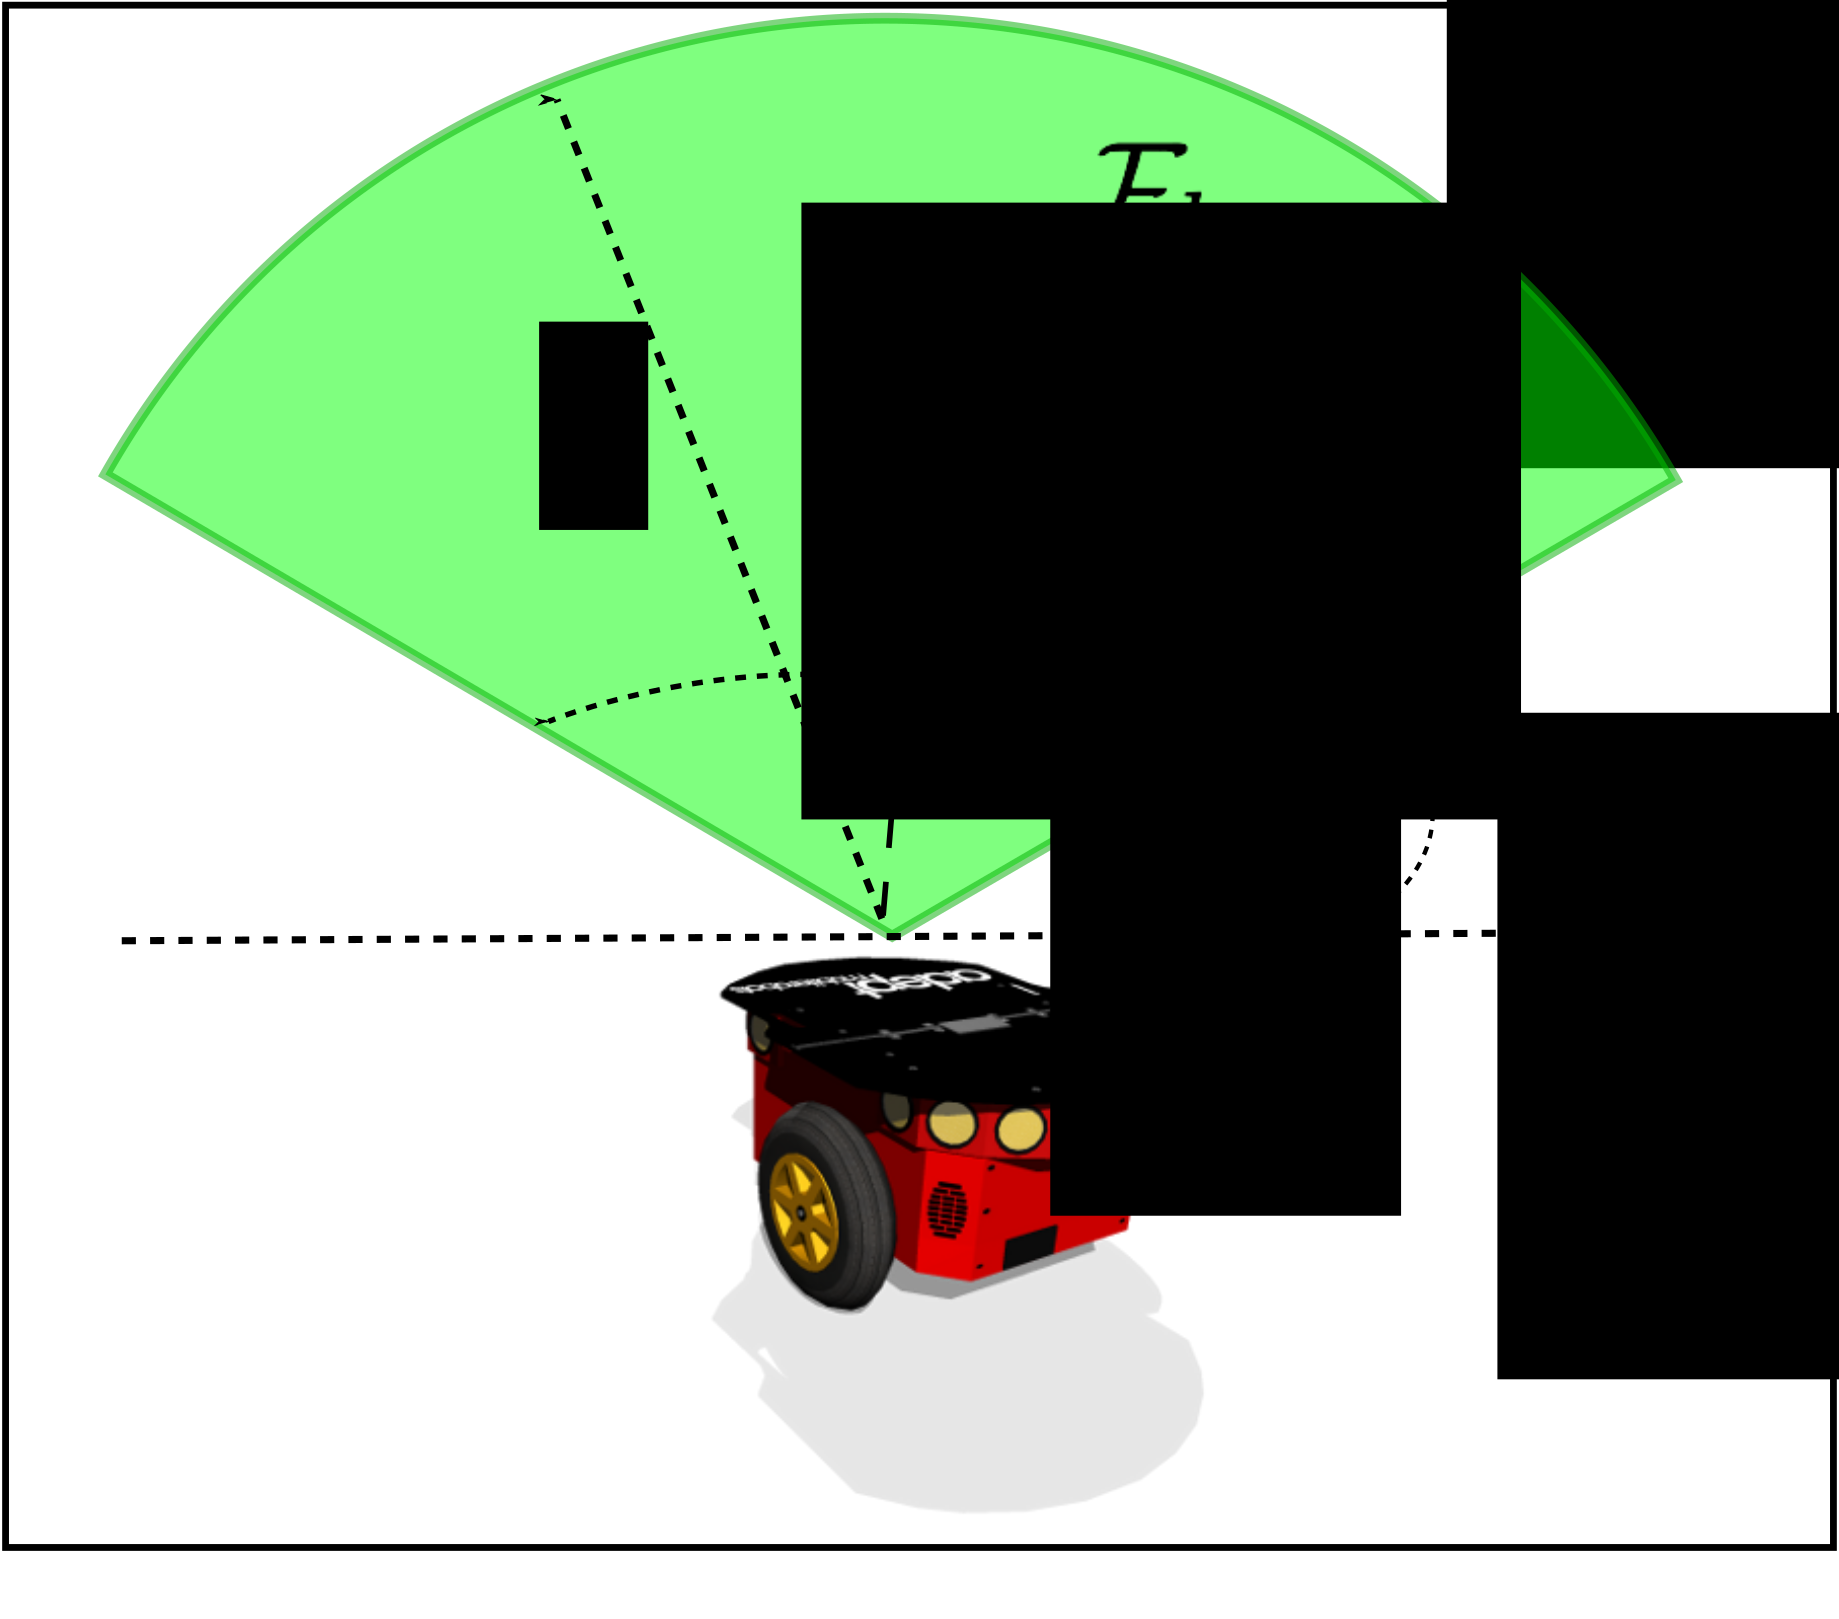
\includegraphics[width=0.28\textwidth]{figures/sensorFOV}
	\caption{Illustration of sensor's sensing domain $\mathcal{F}_k$. The sensing range is $r$ and the sensing angle is $[\theta_1,\theta_2]$. $v$ represents the vector from the sensor origin to the target position.}
	\label{fig:FOV}
\end{figure}


\subsection{Path Planning for Target Search and Tracking}
We formulate the path planning problem using the model predictive control framework. 
MPC is a suitable method for this problem.
This is because the target position constantly gets updated as new sensor measurement is obtained and MPC can utilize the updated target information to re-generate a path at each time instance. 
The MPC-based path planner with planning horizon $N$ can be formulated as:
\begin{subequations}
	\begin{align}
	\min_{u_{1:N}}\; & J(b_{1:N+1},u_{1:N})\\
	\text{s.t. }\; & x^r_{k+1}=f(x^r_k,u^r_k),\\
	& b_{k+1}=g(b_k,u^r_k),\\
	& x^r_{k+1}\in\mathcal{X}, \, u^r_{k+1}\in\mathcal{U},\\
	& k=1,\dots,N,
	\end{align}\label{eqn:MPC}
\end{subequations}
where $J$ is the objective function; $\mathcal{X}$ and $\mathcal{U}$ represent the feasible sets of robot state and control input, consisting of constraints on robot speed, steering rate and linear acceleration.

\begin{figure}
	\centering
	\includegraphics[width=0.28\textwidth]{figures/FOV_function}
	\caption{Illustration of the bell-shaped function for approximating $\gamma_k$. In this example, parameters take the following values: $\tilde{\theta}_k=0,\:\theta_0=\pi/3,\:\alpha_1=1,\:\alpha_2=10$.}
	\label{fig:3d-gamma}
\end{figure}

Information-theoretic measures have been proven to be effective metrics for path planning in information gathering \cite{bourgault2006optimal,ryan2010particle,hoffmann2010mobile,atanasov2015distributed}. 
To drive the robot to configurations in which the sensor can effectively obtain target information, we choose the cumulative entropy and the distance between the robot and predicted target position as the objective function.
%, i.e.
%\begin{equation}
%J(b_{1:N+1},u_{1:N})=\sum\limits_{i=1}^{N} w_1H(b_{i+1})+w_2\|x^t_{i+1}-x^r_{i+1}\|^2
%\end{equation}
%, $H(\hat{x}^t_1)-H(\hat{x}^t_{k+1})$, for the planning horizon. 
%Since $H(\hat{x}^t_1)$ depends only on the target estimation at the current time and is not affected by control input of the robot, it is equivalently to minimizing $H(\hat{x}^t_{k+1})$.
Because of the linear Gaussian noise assumption in the target model and measurement model, target uncertainty follows a Gaussian distribution. 
%According to the entropy of a multivariate normal distribution \cite{information theory book}, 
Therefore, the entropy at $k$ is $H(b_{k}) = \frac{k}{2} (1 + \ln (2\pi)) + \frac{1}{2} \ln |P_{k|k}|$ (\cite{mackay2003information}).
Minimizing a determinant can incur large computation burden for an optimization problem. 
Therefore, we utilize the relation
$|A|^{\frac{1}{n}}\leq \frac{1}{n}tr(A)$ for a positive definite matrix $A$ and define the objective function of the MPC problem as:
\begin{equation*}
J(b_{1:N+1})=\sum\limits_{i=1}^{N} w_1tr(P_{i+1|i+1})+w_2\|x^t_{i+1}-x^r_{i+1}\|^2,
\end{equation*}
where $tr(P_{k|k})$ is the trace of the matrix $P_{k|k}$.
%In the predictive horizon, it is undetermined whether the measurement of target can be obtained or not.
%Therefore, sensor FOV needs to be defined and $\gamma_K$ needs to be represented in the form that can be utilized by the MPC problem. 

The binary variable $\gamma_{k}$ (\Cref{eqn:gamma_indicator}) is a discontinuous function of the robot and target states, which is inconvenient for an optimization problem that usually requires differentiability of functions in it.
Therefore we approximate $\gamma_{k}$ as a product of two bell-shaped differentiable functions, corresponding to bounds on sensing range and angle:
%take the similar approach as in \cite{patil2014gaussian} to use the sigmoid function for approximating $\gamma_{k+1}$.
%A typical camera sensor FOV can be modeled as a sector (\cref{fig:FOV}).
%We use a sigmoid function to approximate its boundary:
\begin{equation}\label{eqn:gamma}
\begin{split}
\gamma_{k}&\approx \frac{1}{1+\alpha_1\|[x^t_{1,k},x^t_{2,k}]-[x^r_{1,k},x^r_{2,k}]\|_2^2}\times\\
&\quad\frac{1}{1+\exp{\left\lbrace-\alpha_2(\cos(\theta^r_k-\tilde{\theta}_k)-\cos(\theta_0))\right\rbrace}},
\end{split}
\end{equation}
where $\tilde{\theta}_k=\angle([x^t_{1,k},x^t_{2,k}]-[x^r_{1,k},x^r_{2,k}])$ is the direction angle from the sensor position to target position; $\theta_0=\frac{\theta_2-\theta_1}{2}$ is half of the sensing angle; $\alpha_1$ and $\alpha_2$ are tunning parameters that controls the shape of the function. 
\Cref{eqn:gamma} can be interpreted as follows:
when the robot is close to the target, it is more likely that the target can be detected; besides, the closer the target direction aligns with the center direction of the sensor, the higher possibility that the target will get detected.
\Cref{fig:3d-gamma} shows the shape of $\gamma_k$.

\begin{figure}
	\centering
	\begin{subfigure}[b]{0.23\textwidth}
		\includegraphics[width=\textwidth]{figures/test1_1}
		%		\caption{}
	\end{subfigure}
	\begin{subfigure}[b]{0.23\textwidth}
		\includegraphics[width=\textwidth]{figures/test1_2}
		%		\caption{}
	\end{subfigure}
	\par\bigskip
	\begin{subfigure}[b]{0.23\textwidth}
		\includegraphics[width=\textwidth]{figures/test1_3}
		%		\caption{}
	\end{subfigure}
	\begin{subfigure}[b]{0.23\textwidth}
		\includegraphics[width=\textwidth]{figures/test1_4}
		%		\caption{}
	\end{subfigure}
	\caption{Intermediate steps of search and tracking. Green dashed sector represents the sensor's sensing domain and the blue dashed circle show the uncertainty of the target position (based on diagonal elements of $\sqrt{P_{k|k}}$). Red and blue lines correspond to the trajectories of the robot and target.}
	\label{fig:test1}
\end{figure}

\subsection{Sequential Planning}
%Due to the coupling between robot state and target position in \Cref{eqn:gamma}, solving the nonlinear MPC problem is time consuming. 
Directly solving the MPC problem in \Cref{eqn:MPC} is time consuming, mainly due to the coupling of robot and target state in $\gamma_k$, as defined in \Cref{eqn:gamma}.
To reduce the computation burden for real-time applications, we make several relaxation to the original MPC problem.
To be specific, in the predictive horizon, the target position is assumed to change following \Cref{eqn:target_motion_model} but without noise, starting from the estimated target position at the beginning of the prediction. 
This is equivalent to predicting target position using \Cref{eqn:KF_pred_x} but without updating step (\Cref{eqn:KF_upd_x}). 
This is a reasonable assumption for MPC framework. 
In fact, because of the stochasticity of target motion and sensor measurement process, it is difficult to accurately predict the evolution of the environment state for a long horizon. 
The benefit of MPC is that it will takes into account the newly received information about the target and then utilize it to update the path at each time step. 
This can compensate for inaccuracy caused by using a simple model to predict target position in the predictive horizon.

We also devise a two-step process to further reduce the computation burden for the MPC problem. 
In the first step, we only consider the limited sensing range of the sensor, assuming a full sensing angle. 
In this step, $\gamma_k$ is equivalent to the first multiplier in \Cref{eqn:gamma}.
With this simplified $\gamma_k$, the MPC computes a reference trajectory of the robot.
Utilizing the generated reference trajectory, the heading angle of sensor $\hat{\theta}_k$ at each predicted time can be computed. 
In the second step, MPC is solved again but with the full expression of $\gamma_k$, in which $\hat{\theta}_k$ takes the value from the first step.
The benefits of conducting this sequential two-step planning process lies in that computing the reference trajectory in the first step generates the reference heading angle of the robot, which reduces the computation burden when later a full version of MPC is solved.

\section{Simulation}\label{sec:sim}

\begin{figure}
	\centering
	\begin{subfigure}[b]{0.23\textwidth}
		\includegraphics[width=\textwidth]{figures/test2}
%		\caption{}
	\end{subfigure}
	\begin{subfigure}[b]{0.23\textwidth}
		\includegraphics[width=\textwidth]{figures/test3}
%		\caption{}
	\end{subfigure}
		\par\bigskip
	\begin{subfigure}[b]{0.23\textwidth}
		\includegraphics[width=\textwidth]{figures/test4}
%		\caption{}
	\end{subfigure}
	\begin{subfigure}[b]{0.24\textwidth}
		\includegraphics[width=\textwidth]{figures/trace_comparison}
%		\caption{}
	\end{subfigure}
	\caption{First three figures show the final steps of search and tracking mission in three different scenarios. The initial estimated target position is set to be the true position. The last figure shows the trace of $P_{k|k}$ at each time step for all four scenarios.}
	\label{fig:other test}
\end{figure}

%\begin{tabular}{|c|c|c|c|c|c|}
%	\hline
%	$a (m/s^2)$ & $[-3,1]$ & $v(m/s)$ & $[0,3]$ & $w(rad/s)$ & $[-\frac{\pi}{4},\frac{\pi}{4}]$\\
%	\hline
%\end{tabular}

We have tested the algorithm on different scenarios. 
Each scenario consists of a mobile robot equipped with a camera and a moving target in a $50m\times 50m$ field.
The initial position of the target is different in each scenario while the robot starts from the same position.
The robot has a maximum speed of $3m/s$ with the acceleration range $[-3m/{s^2},1m/{s^2}]$ and the angular velocity range $[-\frac{\pi}{4},\frac{\pi}{4}]$.
The sensing range $r=5m$ and the sensing angle is $60\degree$.
Target model $A$ and measurement model $C$ are assumed to be identity matrices, with the noise $R=\begin{bmatrix}
1& 0\\0 &1
\end{bmatrix}$ and $Q=\begin{bmatrix}
0.01& 0\\0 &0.01
\end{bmatrix}$.
The value of $B$ varies among different scenarios.

\Cref{fig:test1} shows the intermediate search and tracking steps of a test scenario.
At the beginning, the robot starts from the lower left corner and the target is at the upper right corner.
The estimated target position is initialized as the target's true position but with a large uncertainty.
The robot then moves towards the target by using the control input computed from the MPC problem (\Cref{eqn:MPC}).
At step $21$, the robot successfully detects the target and thus the uncertainty significantly shrinks.
The robot then keeps tracking the target and the uncertainty is further reduced, as the figure of Step $50$ shows.

\begin{figure}
	\centering
	\begin{subfigure}[b]{0.23\textwidth}
		\includegraphics[width=\textwidth]{figures/test1_offset}
		%		\caption{}
	\end{subfigure}
	\begin{subfigure}[b]{0.23\textwidth}
		\includegraphics[width=\textwidth]{figures/test2_offset}
		%		\caption{}
	\end{subfigure}
	\par\bigskip
	\begin{subfigure}[b]{0.23\textwidth}
		\includegraphics[width=\textwidth]{figures/test3_offset}
		%		\caption{}
	\end{subfigure}
	\begin{subfigure}[b]{0.22\textwidth}
		\includegraphics[width=\textwidth]{figures/trace_comparison_offset}
		%		\caption{}
	\end{subfigure}
	\caption{First three figures show the final steps in three  different scenarios. The initial estimated target position is different from the true position. The last figure shows the trace of $P_{k|k}$ at each time step of these scenarios.}
	\label{fig:test_offset}
\end{figure}

Robot and target trajectories in some other test scenarios are shown in \Cref{fig:other test}.
The lower right figure in \Cref{fig:other test} shows the trace of the covariance matrix of the target position.
As expected, uncertainty keeps increasing at the beginning since the target is not found and thus no uncertainty reduction can be conducted by Kalman filter.
Once the target is within the sensor's sensing domain, uncertainty drops significantly since Kalman filter is able to use measurements to improve the estimation of the target position.
The robot then keeps measuring the target position and the uncertainty continues being reduced.
Fluctuation of the trace can also be observed in later part of the search and tracking.
This is mainly due to the fact that the target moves in a stochastic manner and therefore there exists some cases that the target falls out of the sensing domain.
However, the robot is able to adjust its sensor and keep the target in its sensing domain again.
These figures shows that the robot successfully detects the target and then keeps tracking it afterwards in all considered cases using the presented approach.

We have also set the initial estimated target position to be different from the true position, which adds more complexity to the problem. 
Results on three scenarios from \Cref{fig:test1,fig:other test} are presented in \Cref{fig:test_offset}.
It shows that the robot is able to find the target and track it in spite of inaccurate initial estimation.
However, we also notice that, when the initial estimated position is far from the true position, it is difficult for the robot to find the target.
This is not unexpected since in current formulation the estimated target position is propagated using noise-free system model but without correction if no measurement is received.
As \cite{sinopoli2004kalman} indicated, when measurement arrival rate is below certain threshold, the Kalman filter \Cref{eqn:KF} cannot converge.


\section{CONCLUSION}\label{sec:conclu}
In this work, we propose a model predictive control (MPC)-based path planning approach for a ground mobile robot to autonomously search and track a moving target.
%Different from previous works that relies on numerical integration for evaluating the objective function, we developed a closed-form expression, which can greatly reduce the computation burden of solving MPC.
We consider the effects of sensor's limited sensing domain in the predictive horizon by utilizing the modified Kalman filter for handling intermittent measurements.
To deal with the discontinuity caused by limited sensing domain, we propose a bell-shaped function to approximate the sensing domain's boundary.
A two-step sequential planning approach is then developed for solving the MPC problem.
Simulation results have demonstrated the effectiveness of the proposed path planning algorithm in searching and tracking the target.

Though this work achieves good results, we realize some limitations that should be addressed in our future work. 
First, the developed approach relies on the assumption of Gaussian distribution of target uncertainty and is therefore restricted to linear target model and sensor measurement model. 
Methods for general nonlinear dynamic systems need to be developed.
%In \cite{patil2014gaussian}, Extended Kalman filter was used to deal with this issue.
%However, the Gaussian distribution assumption in that work also limits its generalizability.
Second, as discussed in \Cref{sec:sim}, non-convergence can happen if the initial estimation of target position is far from the true value.
%when measurement arrival rate is below a certain threshold, as \cite{sinopoli2004kalman} indicated, Kalman filter is not able to converge. 
Some general nonlinear filters, such as Bayes filter and Particle filter, can therefore be used to improve the robustness of the filtering result.
Lastly, when there exist obstacles in the environment, occlusion may happen that affects the sensor measurement process. 
Taking into account the occlusion in the planning process is our ongoing work.


\addtolength{\textheight}{-14cm}%{-12cm}   % This command serves to balance the column lengths
                                  % on the last page of the document manually. It shortens
                                  % the textheight of the last page by a suitable amount.
                                  % This command does not take effect until the next page
                                  % so it should come on the page before the last. Make
                                  % sure that you do not shorten the textheight too much.

%%%%%%%%%%%%%%%%%%%%%%%%%%%%%%%%%%%%%%%%%%%%%%%%%%%%%%%%%%%%%%%%%%%%%%%%%%%%%%%%



%%%%%%%%%%%%%%%%%%%%%%%%%%%%%%%%%%%%%%%%%%%%%%%%%%%%%%%%%%%%%%%%%%%%%%%%%%%%%%%%



%%%%%%%%%%%%%%%%%%%%%%%%%%%%%%%%%%%%%%%%%%%%%%%%%%%%%%%%%%%%%%%%%%%%%%%%%%%%%%%%
%\section*{APPENDIX}
%
%Appendixes should appear before the acknowledgment.

%\section*{ACKNOWLEDGMENT}
%%This work is supported by the Embedded Humans: Provably Correct Decision Making for Networks of Humans and Unmanned Systems project, a MURI project funded by the Office of Naval Research.
%The authors gratefully acknowledges the Office of Naval Research for supporting the research described in this paper. 
%They would also like to thank Yuting Wei in the Department of Statistics, UC Berkeley for her sincere help and fruitful discussion on the consistency proof.

%The preferred spelling of the word �acknowledgment� in America is without an �e� after the �g�. Avoid the stilted expression, �One of us (R. B. G.) thanks . . .�  Instead, try �R. B. G. thanks�. Put sponsor acknowledgments in the unnumbered footnote on the first page.



%%%%%%%%%%%%%%%%%%%%%%%%%%%%%%%%%%%%%%%%%%%%%%%%%%%%%%%%%%%%%%%%%%%%%%%%%%%%%%%%
\bibliographystyle{IEEEtran}
%\bibliographystyle{bibtex}
\bibliography{references}

\end{document}
